% Options for packages loaded elsewhere
\PassOptionsToPackage{unicode}{hyperref}
\PassOptionsToPackage{hyphens}{url}
\PassOptionsToPackage{dvipsnames,svgnames,x11names}{xcolor}
%
\documentclass[
  letterpaper,
  DIV=11,
  numbers=noendperiod]{scrartcl}

\usepackage{amsmath,amssymb}
\usepackage{iftex}
\ifPDFTeX
  \usepackage[T1]{fontenc}
  \usepackage[utf8]{inputenc}
  \usepackage{textcomp} % provide euro and other symbols
\else % if luatex or xetex
  \usepackage{unicode-math}
  \defaultfontfeatures{Scale=MatchLowercase}
  \defaultfontfeatures[\rmfamily]{Ligatures=TeX,Scale=1}
\fi
\usepackage{lmodern}
\ifPDFTeX\else  
    % xetex/luatex font selection
\fi
% Use upquote if available, for straight quotes in verbatim environments
\IfFileExists{upquote.sty}{\usepackage{upquote}}{}
\IfFileExists{microtype.sty}{% use microtype if available
  \usepackage[]{microtype}
  \UseMicrotypeSet[protrusion]{basicmath} % disable protrusion for tt fonts
}{}
\makeatletter
\@ifundefined{KOMAClassName}{% if non-KOMA class
  \IfFileExists{parskip.sty}{%
    \usepackage{parskip}
  }{% else
    \setlength{\parindent}{0pt}
    \setlength{\parskip}{6pt plus 2pt minus 1pt}}
}{% if KOMA class
  \KOMAoptions{parskip=half}}
\makeatother
\usepackage{xcolor}
\setlength{\emergencystretch}{3em} % prevent overfull lines
\setcounter{secnumdepth}{-\maxdimen} % remove section numbering
% Make \paragraph and \subparagraph free-standing
\ifx\paragraph\undefined\else
  \let\oldparagraph\paragraph
  \renewcommand{\paragraph}[1]{\oldparagraph{#1}\mbox{}}
\fi
\ifx\subparagraph\undefined\else
  \let\oldsubparagraph\subparagraph
  \renewcommand{\subparagraph}[1]{\oldsubparagraph{#1}\mbox{}}
\fi

\usepackage{color}
\usepackage{fancyvrb}
\newcommand{\VerbBar}{|}
\newcommand{\VERB}{\Verb[commandchars=\\\{\}]}
\DefineVerbatimEnvironment{Highlighting}{Verbatim}{commandchars=\\\{\}}
% Add ',fontsize=\small' for more characters per line
\usepackage{framed}
\definecolor{shadecolor}{RGB}{241,243,245}
\newenvironment{Shaded}{\begin{snugshade}}{\end{snugshade}}
\newcommand{\AlertTok}[1]{\textcolor[rgb]{0.68,0.00,0.00}{#1}}
\newcommand{\AnnotationTok}[1]{\textcolor[rgb]{0.37,0.37,0.37}{#1}}
\newcommand{\AttributeTok}[1]{\textcolor[rgb]{0.40,0.45,0.13}{#1}}
\newcommand{\BaseNTok}[1]{\textcolor[rgb]{0.68,0.00,0.00}{#1}}
\newcommand{\BuiltInTok}[1]{\textcolor[rgb]{0.00,0.23,0.31}{#1}}
\newcommand{\CharTok}[1]{\textcolor[rgb]{0.13,0.47,0.30}{#1}}
\newcommand{\CommentTok}[1]{\textcolor[rgb]{0.37,0.37,0.37}{#1}}
\newcommand{\CommentVarTok}[1]{\textcolor[rgb]{0.37,0.37,0.37}{\textit{#1}}}
\newcommand{\ConstantTok}[1]{\textcolor[rgb]{0.56,0.35,0.01}{#1}}
\newcommand{\ControlFlowTok}[1]{\textcolor[rgb]{0.00,0.23,0.31}{#1}}
\newcommand{\DataTypeTok}[1]{\textcolor[rgb]{0.68,0.00,0.00}{#1}}
\newcommand{\DecValTok}[1]{\textcolor[rgb]{0.68,0.00,0.00}{#1}}
\newcommand{\DocumentationTok}[1]{\textcolor[rgb]{0.37,0.37,0.37}{\textit{#1}}}
\newcommand{\ErrorTok}[1]{\textcolor[rgb]{0.68,0.00,0.00}{#1}}
\newcommand{\ExtensionTok}[1]{\textcolor[rgb]{0.00,0.23,0.31}{#1}}
\newcommand{\FloatTok}[1]{\textcolor[rgb]{0.68,0.00,0.00}{#1}}
\newcommand{\FunctionTok}[1]{\textcolor[rgb]{0.28,0.35,0.67}{#1}}
\newcommand{\ImportTok}[1]{\textcolor[rgb]{0.00,0.46,0.62}{#1}}
\newcommand{\InformationTok}[1]{\textcolor[rgb]{0.37,0.37,0.37}{#1}}
\newcommand{\KeywordTok}[1]{\textcolor[rgb]{0.00,0.23,0.31}{#1}}
\newcommand{\NormalTok}[1]{\textcolor[rgb]{0.00,0.23,0.31}{#1}}
\newcommand{\OperatorTok}[1]{\textcolor[rgb]{0.37,0.37,0.37}{#1}}
\newcommand{\OtherTok}[1]{\textcolor[rgb]{0.00,0.23,0.31}{#1}}
\newcommand{\PreprocessorTok}[1]{\textcolor[rgb]{0.68,0.00,0.00}{#1}}
\newcommand{\RegionMarkerTok}[1]{\textcolor[rgb]{0.00,0.23,0.31}{#1}}
\newcommand{\SpecialCharTok}[1]{\textcolor[rgb]{0.37,0.37,0.37}{#1}}
\newcommand{\SpecialStringTok}[1]{\textcolor[rgb]{0.13,0.47,0.30}{#1}}
\newcommand{\StringTok}[1]{\textcolor[rgb]{0.13,0.47,0.30}{#1}}
\newcommand{\VariableTok}[1]{\textcolor[rgb]{0.07,0.07,0.07}{#1}}
\newcommand{\VerbatimStringTok}[1]{\textcolor[rgb]{0.13,0.47,0.30}{#1}}
\newcommand{\WarningTok}[1]{\textcolor[rgb]{0.37,0.37,0.37}{\textit{#1}}}

\providecommand{\tightlist}{%
  \setlength{\itemsep}{0pt}\setlength{\parskip}{0pt}}\usepackage{longtable,booktabs,array}
\usepackage{calc} % for calculating minipage widths
% Correct order of tables after \paragraph or \subparagraph
\usepackage{etoolbox}
\makeatletter
\patchcmd\longtable{\par}{\if@noskipsec\mbox{}\fi\par}{}{}
\makeatother
% Allow footnotes in longtable head/foot
\IfFileExists{footnotehyper.sty}{\usepackage{footnotehyper}}{\usepackage{footnote}}
\makesavenoteenv{longtable}
\usepackage{graphicx}
\makeatletter
\def\maxwidth{\ifdim\Gin@nat@width>\linewidth\linewidth\else\Gin@nat@width\fi}
\def\maxheight{\ifdim\Gin@nat@height>\textheight\textheight\else\Gin@nat@height\fi}
\makeatother
% Scale images if necessary, so that they will not overflow the page
% margins by default, and it is still possible to overwrite the defaults
% using explicit options in \includegraphics[width, height, ...]{}
\setkeys{Gin}{width=\maxwidth,height=\maxheight,keepaspectratio}
% Set default figure placement to htbp
\makeatletter
\def\fps@figure{htbp}
\makeatother

\KOMAoption{captions}{tableheading}
\makeatletter
\makeatother
\makeatletter
\makeatother
\makeatletter
\@ifpackageloaded{caption}{}{\usepackage{caption}}
\AtBeginDocument{%
\ifdefined\contentsname
  \renewcommand*\contentsname{Table of contents}
\else
  \newcommand\contentsname{Table of contents}
\fi
\ifdefined\listfigurename
  \renewcommand*\listfigurename{List of Figures}
\else
  \newcommand\listfigurename{List of Figures}
\fi
\ifdefined\listtablename
  \renewcommand*\listtablename{List of Tables}
\else
  \newcommand\listtablename{List of Tables}
\fi
\ifdefined\figurename
  \renewcommand*\figurename{Figure}
\else
  \newcommand\figurename{Figure}
\fi
\ifdefined\tablename
  \renewcommand*\tablename{Table}
\else
  \newcommand\tablename{Table}
\fi
}
\@ifpackageloaded{float}{}{\usepackage{float}}
\floatstyle{ruled}
\@ifundefined{c@chapter}{\newfloat{codelisting}{h}{lop}}{\newfloat{codelisting}{h}{lop}[chapter]}
\floatname{codelisting}{Listing}
\newcommand*\listoflistings{\listof{codelisting}{List of Listings}}
\makeatother
\makeatletter
\@ifpackageloaded{caption}{}{\usepackage{caption}}
\@ifpackageloaded{subcaption}{}{\usepackage{subcaption}}
\makeatother
\makeatletter
\@ifpackageloaded{tcolorbox}{}{\usepackage[skins,breakable]{tcolorbox}}
\makeatother
\makeatletter
\@ifundefined{shadecolor}{\definecolor{shadecolor}{rgb}{.97, .97, .97}}
\makeatother
\makeatletter
\makeatother
\makeatletter
\makeatother
\ifLuaTeX
  \usepackage{selnolig}  % disable illegal ligatures
\fi
\IfFileExists{bookmark.sty}{\usepackage{bookmark}}{\usepackage{hyperref}}
\IfFileExists{xurl.sty}{\usepackage{xurl}}{} % add URL line breaks if available
\urlstyle{same} % disable monospaced font for URLs
\hypersetup{
  pdftitle={Running a Simulation Study},
  colorlinks=true,
  linkcolor={blue},
  filecolor={Maroon},
  citecolor={Blue},
  urlcolor={Blue},
  pdfcreator={LaTeX via pandoc}}

\title{Running a Simulation Study}
\author{}
\date{}

\begin{document}
\maketitle
\ifdefined\Shaded\renewenvironment{Shaded}{\begin{tcolorbox}[enhanced, boxrule=0pt, interior hidden, borderline west={3pt}{0pt}{shadecolor}, sharp corners, frame hidden, breakable]}{\end{tcolorbox}}\fi

\hypertarget{an-example-of-a-statistical-simulation}{%
\subsection{An Example of a statistical
simulation}\label{an-example-of-a-statistical-simulation}}

Small scale simulation study to investigate impact of measurement error
on (continuous) exposure and/or (continuous) confounding variable. In
epidemiological studies of the relation between an exposure and an
outcome, this relation is often estimated using regression analysis. As
an example, we consider a study of the association between glycated
haemoglobin (HbA1c) levels and systolic blood pressure assessed using
linear regression. Data from 5092 subjects in the 2015--2016 National
Health and Nutrition Examination Survey (NHANES) are used to obtain an
estimate of the effect of HbA1c on systolic blood pressure, while
adjusting for age, gender and body mass index (BMI).

\hypertarget{analysis}{%
\subsection{Analysis}\label{analysis}}

After adjustment for age and gender, it was estimated that HbA1c
increases systolic blood pressure by 1.13 mmHg (95\% CI 0.73 to 1.52)
per unit increase in HbA1c.

\begin{Shaded}
\begin{Highlighting}[]
\FunctionTok{summary}\NormalTok{(}\FunctionTok{lm}\NormalTok{(bp }\SpecialCharTok{\textasciitilde{}}\NormalTok{ HbA1C }\SpecialCharTok{+}\NormalTok{ age }\SpecialCharTok{+} \FunctionTok{as.factor}\NormalTok{(sex), }\AttributeTok{data=}\NormalTok{dc))}
\end{Highlighting}
\end{Shaded}

\begin{verbatim}

Call:
lm(formula = bp ~ HbA1C + age + as.factor(sex), data = dc)

Residuals:
Systolic: Blood pres (1st rdg) mm Hg 
    Min      1Q  Median      3Q     Max 
-49.887 -10.509  -1.378   8.491 107.583 

Coefficients:
                Estimate Std. Error t value Pr(>|t|)    
(Intercept)     98.75149    1.21418  81.332  < 2e-16 ***
HbA1C            1.12638    0.20291   5.551 2.98e-08 ***
age              0.44486    0.01284  34.648  < 2e-16 ***
as.factor(sex)2 -3.24792    0.45164  -7.191 7.34e-13 ***
---
Signif. codes:  0 '***' 0.001 '**' 0.01 '*' 0.05 '.' 0.1 ' ' 1

Residual standard error: 16.1 on 5088 degrees of freedom
Multiple R-squared:  0.2305,    Adjusted R-squared:   0.23 
F-statistic:   508 on 3 and 5088 DF,  p-value: < 2.2e-16
\end{verbatim}

\begin{Shaded}
\begin{Highlighting}[]
\FunctionTok{confint}\NormalTok{(}\FunctionTok{lm}\NormalTok{(bp }\SpecialCharTok{\textasciitilde{}}\NormalTok{ HbA1C }\SpecialCharTok{+}\NormalTok{ age }\SpecialCharTok{+} \FunctionTok{as.factor}\NormalTok{(sex), }\AttributeTok{data=}\NormalTok{dc))}
\end{Highlighting}
\end{Shaded}

\begin{verbatim}
                     2.5 %      97.5 %
(Intercept)     96.3711755 101.1317982
HbA1C            0.7285836   1.5241825
age              0.4196932   0.4700355
as.factor(sex)2 -4.1333281  -2.3625106
\end{verbatim}

Additional adjustment for BMI resulted in a considerable change in the
effect estimate: HbA1c was estimated to increase blood pressure by 0.75
mmHg (95\% CI 0.35 to 1.16) per unit increase in HbA1c.

\begin{Shaded}
\begin{Highlighting}[]
\FunctionTok{summary}\NormalTok{(}\FunctionTok{lm}\NormalTok{(bp }\SpecialCharTok{\textasciitilde{}}\NormalTok{ HbA1C }\SpecialCharTok{+}\NormalTok{ bmi }\SpecialCharTok{+}\NormalTok{ age }\SpecialCharTok{+} \FunctionTok{as.factor}\NormalTok{(sex), }\AttributeTok{data=}\NormalTok{dc))}
\end{Highlighting}
\end{Shaded}

\begin{verbatim}

Call:
lm(formula = bp ~ HbA1C + bmi + age + as.factor(sex), data = dc)

Residuals:
Systolic: Blood pres (1st rdg) mm Hg 
    Min      1Q  Median      3Q     Max 
-51.068 -10.251  -1.504   8.264 107.410 

Coefficients:
                Estimate Std. Error t value Pr(>|t|)    
(Intercept)     92.65583    1.39320  66.506  < 2e-16 ***
HbA1C            0.75177    0.20596   3.650 0.000265 ***
bmi              0.28632    0.03282   8.724  < 2e-16 ***
age              0.44586    0.01275  34.979  < 2e-16 ***
as.factor(sex)2 -3.63115    0.45049  -8.060  9.4e-16 ***
---
Signif. codes:  0 '***' 0.001 '**' 0.01 '*' 0.05 '.' 0.1 ' ' 1

Residual standard error: 15.98 on 5087 degrees of freedom
Multiple R-squared:  0.2418,    Adjusted R-squared:  0.2412 
F-statistic: 405.7 on 4 and 5087 DF,  p-value: < 2.2e-16
\end{verbatim}

\begin{Shaded}
\begin{Highlighting}[]
\FunctionTok{confint}\NormalTok{(}\FunctionTok{lm}\NormalTok{(bp }\SpecialCharTok{\textasciitilde{}}\NormalTok{ HbA1C }\SpecialCharTok{+}\NormalTok{ bmi }\SpecialCharTok{+}\NormalTok{ age }\SpecialCharTok{+} \FunctionTok{as.factor}\NormalTok{(sex), }\AttributeTok{data=}\NormalTok{dc))}
\end{Highlighting}
\end{Shaded}

\begin{verbatim}
                     2.5 %     97.5 %
(Intercept)     89.9245592 95.3871089
HbA1C            0.3479966  1.1555348
bmi              0.2219815  0.3506673
age              0.4208695  0.4708464
as.factor(sex)2 -4.5143014 -2.7479929
\end{verbatim}

\hypertarget{run-the-simulation-study}{%
\subsection{Run the simulation study}\label{run-the-simulation-study}}

One way to investigate the possible impact of measurement error is
through a small simulation study. For the purpose of this example, the
original recordings in the NHANES data were assumed to be measured
without error. Then, in addition, new artificial variables were created
that represented HbA1c and BMI, but for the situation in which these are
measured with error. To create these variables, measurement error was
artificially added to the exposure variable (HbA1c) and/or the
confounding variable (BMI). These errors were drawn from a normal
distribution with a mean zero and were independent of all variables
considered. The variance of the normal distribution, defining the amount
of measurement error added, was altered for different scenarios.
Scenarios ranged from no measurement error on either HbA1c or BMI
(reference scenario) to 50\% of the variance in HbA1c and/or BMI
attributable to measurement error. To minimise the impact of simulation
error, each scenario was repeated 1000 times and the results were
averaged per scenario over these 1000 repetitions.

\begin{Shaded}
\begin{Highlighting}[]
\NormalTok{ref }\OtherTok{\textless{}{-}} \FunctionTok{lm}\NormalTok{(bp }\SpecialCharTok{\textasciitilde{}}\NormalTok{ HbA1C }\SpecialCharTok{+}\NormalTok{ bmi }\SpecialCharTok{+}\NormalTok{ age }\SpecialCharTok{+} \FunctionTok{as.factor}\NormalTok{(sex), }\AttributeTok{data=}\NormalTok{dc)}\SpecialCharTok{$}\NormalTok{coef[}\DecValTok{2}\NormalTok{]}
\NormalTok{n.sim }\OtherTok{\textless{}{-}} \FloatTok{1e3}
\NormalTok{pb }\OtherTok{\textless{}{-}} \FunctionTok{txtProgressBar}\NormalTok{(}\AttributeTok{min=}\DecValTok{1}\NormalTok{, }\AttributeTok{max=} \FloatTok{1e3}\NormalTok{,}\AttributeTok{style=}\DecValTok{3}\NormalTok{, }\DecValTok{50}\NormalTok{)}
\NormalTok{perc.me.exp }\OtherTok{\textless{}{-}} \FunctionTok{seq}\NormalTok{(}\DecValTok{0}\NormalTok{,.}\DecValTok{5}\NormalTok{,.}\DecValTok{1}\NormalTok{)}
\NormalTok{perc.me.conf}\OtherTok{\textless{}{-}} \FunctionTok{seq}\NormalTok{(}\DecValTok{0}\NormalTok{,.}\DecValTok{5}\NormalTok{,.}\DecValTok{1}\NormalTok{)}
\NormalTok{scenarios }\OtherTok{\textless{}{-}} \FunctionTok{expand.grid}\NormalTok{(perc.me.exp,perc.me.conf)}
\NormalTok{var.exp }\OtherTok{\textless{}{-}} \FunctionTok{var}\NormalTok{(dc}\SpecialCharTok{$}\NormalTok{HbA1C)}
\NormalTok{var.conf }\OtherTok{\textless{}{-}} \FunctionTok{var}\NormalTok{(dc}\SpecialCharTok{$}\NormalTok{bmi)}
\NormalTok{n }\OtherTok{\textless{}{-}} \FunctionTok{dim}\NormalTok{(dc)[}\DecValTok{1}\NormalTok{]}
\NormalTok{beta.hat }\OtherTok{\textless{}{-}} \FunctionTok{matrix}\NormalTok{(}\AttributeTok{ncol=}\FunctionTok{dim}\NormalTok{(scenarios)[}\DecValTok{1}\NormalTok{], }\AttributeTok{nrow=}\NormalTok{n.sim)}



\ControlFlowTok{for}\NormalTok{ (k }\ControlFlowTok{in} \DecValTok{1}\SpecialCharTok{:}\NormalTok{n.sim)\{}
  \FunctionTok{set.seed}\NormalTok{(k)}
  \ControlFlowTok{for}\NormalTok{ (i }\ControlFlowTok{in} \DecValTok{1}\SpecialCharTok{:}\FunctionTok{dim}\NormalTok{(scenarios)[}\DecValTok{1}\NormalTok{])\{}
\NormalTok{    var.me.exp }\OtherTok{\textless{}{-}}\NormalTok{ var.exp}\SpecialCharTok{*}\NormalTok{scenarios[i,}\DecValTok{1}\NormalTok{]}\SpecialCharTok{/}\NormalTok{(}\DecValTok{1}\SpecialCharTok{{-}}\NormalTok{scenarios[i,}\DecValTok{1}\NormalTok{])}
\NormalTok{    var.me.conf }\OtherTok{\textless{}{-}}\NormalTok{ var.conf}\SpecialCharTok{*}\NormalTok{scenarios[i,}\DecValTok{2}\NormalTok{]}\SpecialCharTok{/}\NormalTok{(}\DecValTok{1}\SpecialCharTok{{-}}\NormalTok{scenarios[i,}\DecValTok{2}\NormalTok{])}
\NormalTok{    dc}\SpecialCharTok{$}\NormalTok{HbA1C.me }\OtherTok{\textless{}{-}}\NormalTok{ dc}\SpecialCharTok{$}\NormalTok{HbA1C }\SpecialCharTok{+} \FunctionTok{rnorm}\NormalTok{(}\FunctionTok{dim}\NormalTok{(dc)[}\DecValTok{1}\NormalTok{], }\DecValTok{0}\NormalTok{, }\FunctionTok{sqrt}\NormalTok{(var.me.exp))}
\NormalTok{    dc}\SpecialCharTok{$}\NormalTok{bmi.me }\OtherTok{\textless{}{-}}\NormalTok{ dc}\SpecialCharTok{$}\NormalTok{bmi }\SpecialCharTok{+} \FunctionTok{rnorm}\NormalTok{(}\FunctionTok{dim}\NormalTok{(dc)[}\DecValTok{1}\NormalTok{], }\DecValTok{0}\NormalTok{, }\FunctionTok{sqrt}\NormalTok{(var.me.conf))}
\NormalTok{    beta.hat[k,i] }\OtherTok{\textless{}{-}} \FunctionTok{lm}\NormalTok{(bp }\SpecialCharTok{\textasciitilde{}}\NormalTok{ HbA1C.me }\SpecialCharTok{+}\NormalTok{ age }\SpecialCharTok{+}\NormalTok{ bmi.me }\SpecialCharTok{+} \FunctionTok{as.factor}\NormalTok{(sex), }\AttributeTok{data=}\NormalTok{dc)}\SpecialCharTok{$}\NormalTok{coef[}\DecValTok{2}\NormalTok{]}
    \FunctionTok{setTxtProgressBar}\NormalTok{(pb, k)}
\NormalTok{  \}\}}

\FunctionTok{close}\NormalTok{(pb)}
\end{Highlighting}
\end{Shaded}

\hypertarget{results}{%
\subsection{Results}\label{results}}

Thus figure shows the impact of measurement error on HbA1c and/or BMI on
the estimate of the regression coefficient of HbA1c .The relation
between HbA1c and systolic blood pressure was attenuated when
measurement error was added to HbA1c, but not when measurement error was
added to BMI. The association became stronger as measurement error was
added solely to the confounding variable BMI. The reason for this effect
is that, with increasing levels of measurement error on BMI, adjustment
for the confounding due to BMI becomes less efficient and the effect
estimate gets closer to the unadjusted estimate (1.13 mmHg). Due to
measurement error, a type of residual confounding is introduced. In the
case of measurement error on HbA1c as well as BMI, both phenomena play a
role and may cancel each other out. In this study, measurement error on
HbA1c seemed more influential than measurement error on BMI.

\begin{Shaded}
\begin{Highlighting}[]
\NormalTok{tot.mat }\OtherTok{\textless{}{-}} \FunctionTok{cbind}\NormalTok{(}\DecValTok{100}\SpecialCharTok{*}\NormalTok{scenarios,}\FunctionTok{apply}\NormalTok{(beta.hat,}\DecValTok{2}\NormalTok{,mean))}
\FunctionTok{colnames}\NormalTok{(tot.mat) }\OtherTok{\textless{}{-}} \FunctionTok{c}\NormalTok{(}\StringTok{"me.exp"}\NormalTok{,}\StringTok{"me.conf"}\NormalTok{,}\StringTok{"estimate"}\NormalTok{)}
\FunctionTok{ggplot}\NormalTok{(tot.mat, }\FunctionTok{aes}\NormalTok{(me.exp, me.conf)) }\SpecialCharTok{+}
  \FunctionTok{geom\_tile}\NormalTok{(}\AttributeTok{color=}\StringTok{"white"}\NormalTok{,}\FunctionTok{aes}\NormalTok{(}\AttributeTok{fill =}\NormalTok{ estimate)) }\SpecialCharTok{+}
  \FunctionTok{geom\_text}\NormalTok{(}\FunctionTok{aes}\NormalTok{(}\AttributeTok{label =} \FunctionTok{round}\NormalTok{(estimate, }\DecValTok{2}\NormalTok{))) }\SpecialCharTok{+}
  \FunctionTok{scale\_fill\_gradient2}\NormalTok{(}\AttributeTok{low=}\StringTok{"\#D55E00"}\NormalTok{,}
                       \AttributeTok{mid=}\StringTok{"white"}\NormalTok{,}
                       \AttributeTok{high =} \StringTok{"\#56B4E9"}\NormalTok{, }
                       \AttributeTok{midpoint=}\NormalTok{ref) }\SpecialCharTok{+}
  \FunctionTok{labs}\NormalTok{(}\AttributeTok{x=}\FunctionTok{paste}\NormalTok{(}\StringTok{"\% of total variance of HbA1c due to measurement error"}\NormalTok{), }
       \AttributeTok{y=}\FunctionTok{paste}\NormalTok{(}\StringTok{"\% of total variance of BMI due to measurement error"}\NormalTok{)) }\SpecialCharTok{+}
  \FunctionTok{coord\_equal}\NormalTok{()}\SpecialCharTok{+}
  \FunctionTok{scale\_y\_continuous}\NormalTok{(}\AttributeTok{breaks=}\FunctionTok{unique}\NormalTok{(tot.mat[,}\DecValTok{1}\NormalTok{]))}\SpecialCharTok{+}
  \FunctionTok{scale\_x\_continuous}\NormalTok{(}\AttributeTok{breaks=}\FunctionTok{unique}\NormalTok{(tot.mat[,}\DecValTok{1}\NormalTok{]))}\SpecialCharTok{+}
  \FunctionTok{theme}\NormalTok{(}\AttributeTok{panel.background =} \FunctionTok{element\_rect}\NormalTok{(}\AttributeTok{fill=}\StringTok{\textquotesingle{}white\textquotesingle{}}\NormalTok{, }\AttributeTok{colour=}\StringTok{\textquotesingle{}grey\textquotesingle{}}\NormalTok{), }
        \AttributeTok{plot.title=}\FunctionTok{element\_text}\NormalTok{(}\AttributeTok{hjust=}\DecValTok{0}\NormalTok{), }
        \AttributeTok{axis.ticks=}\FunctionTok{element\_blank}\NormalTok{(),}
        \AttributeTok{axis.title=}\FunctionTok{element\_text}\NormalTok{(}\AttributeTok{size=}\DecValTok{12}\NormalTok{),}
        \AttributeTok{axis.text=}\FunctionTok{element\_text}\NormalTok{(}\AttributeTok{size=}\DecValTok{10}\NormalTok{),}
        \AttributeTok{legend.title=}\FunctionTok{element\_text}\NormalTok{(}\AttributeTok{size=}\DecValTok{12}\NormalTok{),}
        \AttributeTok{legend.text=}\FunctionTok{element\_text}\NormalTok{(}\AttributeTok{size=}\DecValTok{10}\NormalTok{))}
\end{Highlighting}
\end{Shaded}

\begin{figure}[H]

{\centering 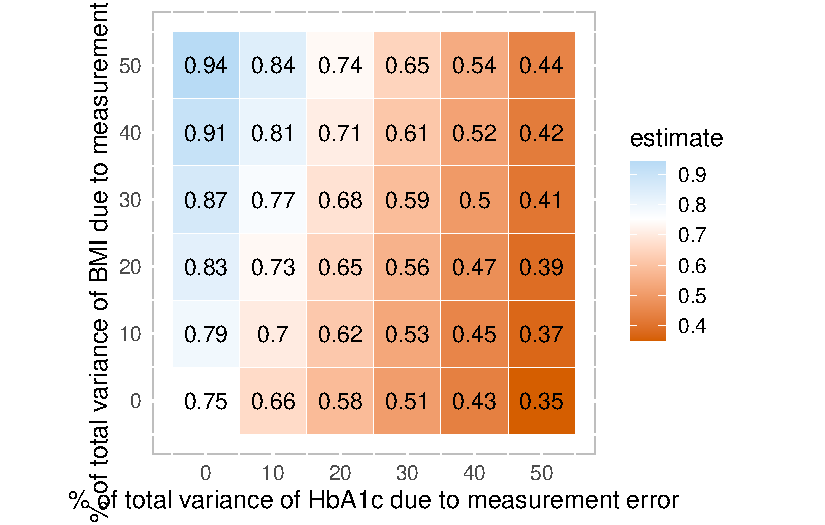
\includegraphics{Running_a_Simulation_Study_files/figure-pdf/unnamed-chunk-5-1.pdf}

}

\end{figure}



\end{document}
